\documentclass{standalone}

\usepackage[dvipsnames]{xcolor}
\usepackage{pgfplots}
\usepackage{tikz}

\usepgfplotslibrary{statistics}

\begin{document}

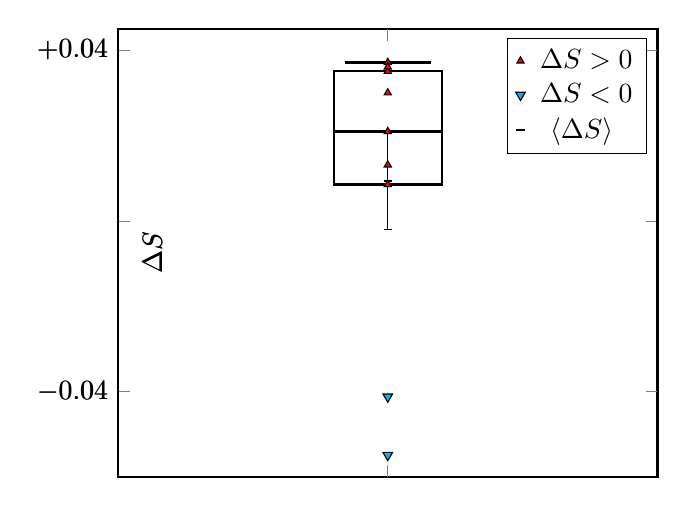
\begin{tikzpicture}


\begin{axis}[
	/pgfplots/boxplot/box extend=0.40,
	thick,
	scaled ticks=false,
	xmin = 0, xmax = 2,
	ymax = 0.045, ymin =-0.060,
	xtick={1},
	ytick = {0.04, 0.00, -0.04},
	xticklabels={\,},
	yticklabels = {$+0.04$, \,, $-0.04$},
	y label style={at={(axis description cs:0.1,.5)}},
	x label style={at={(axis description cs:0.5,0.0125)}},
	ylabel = $\Delta S$,
	boxplot/draw direction=y]
	\addplot [
		thick,
		boxplot,
		mark=triangle*,
		mark size = 0.25pt,
		boxplot prepared={
			lower whisker=0.00852,
			lower quartile=0.00852, % Q1
			median=0.02095,
			upper quartile=0.03504, % Q3
			upper whisker=0.03711,
			},
		] table [row sep=\\,y index=0] {
			-0.04119\\ -0.05487\\ % outlier
	};

\end{axis}

\begin{axis}
	[
	scaled ticks=false,
	xmin = 0, xmax = 2,
	ymax = 0.045, ymin =-0.060,
	xtick={1},
	ytick = {0.04, -0.04},
	xticklabels={\,},
	yticklabels = {$+0.04$, $-0.04$},
	y label style={at={(axis description cs:0.1,.5)}},
	x label style={at={(axis description cs:0.5,0.0125)}},
	ylabel = $\Delta S$,
	legend entries={~$\Delta S > 0$, ~$\Delta S < 0$, $\langle\Delta S\rangle$},
	]

% ---------------------------------------------------------------
%                         Data points 
% ---------------------------------------------------------------
	\addplot[
	color = black,
	fill = red,
	mark = triangle*,
	mark size = 1.5pt,
	only marks
	] coordinates {
	( 1, 0.02095 )
	( 1, 0.01312 )
	( 1, 0.00852 )
	( 1, 0.03711 )
	( 1, 0.03504)
	( 1, 0.03 )
	( 1, 0.03606 )
	};

% The two points in the \Delta S < 0 zone
	\addplot[
	color = black,
	fill = ProcessBlue,
	mark = triangle*,
	mark options={rotate=180},
	mark size = 2.0pt,
	only marks
	] coordinates {
	( 1, -0.04119 )
	( 1, -0.05487 )	
	};	

% Error bar 
	\addplot+[
	color=black, 
	only marks, 
	mark=-,
	mark size = 1.5pt,
	thick,
	error bars/.cd,
	y dir=both, y explicit,]
	coordinates {
	( 1, 0.00941 ) +- (0, 0.01142)
	};

\end{axis}

\end{tikzpicture}

\end{document}
